%  compress using: gs -sDEVICE=pdfwrite -dCompatibilityLevel=1.4 -dNOPAUSE -dQUIET -dBATCH      -sOutputFile=foo-compressed.pdf SeismicDrones.pdf
\documentclass[letterpaper, 10 pt, conference]{ieeeconf}
%\IEEEoverridecommandlockouts
%\documentclass[conference]{IEEEtran}
\newcommand{\subparagraph}{}
\usepackage{epsfig,graphicx,cite}
\usepackage{psfrag}
\usepackage[small,compact]{titlesec}
\usepackage{wrapfig}
\usepackage{mathrsfs}
\usepackage{bm}
\usepackage{cite,url,subfigure,epsfig,graphicx}
\usepackage{verbatim,amsfonts,amsmath,amssymb}
\usepackage{fancyhdr}
\usepackage{mathbbold}
\usepackage{bbm}
\usepackage{mathrsfs}
\usepackage{amsfonts}
\usepackage{cite,url,subfigure,epsfig,graphicx}
\usepackage{amssymb,amsmath,bm,makecell}
\usepackage{indentfirst}
\usepackage{overpic}
\newcommand{\figwid}{0.22\columnwidth}

\usepackage{amsmath}
\usepackage{algorithm}
\usepackage[noend]{algpseudocode}

\usepackage[T1]{fontenc}
\usepackage[utf8]{inputenc}
\usepackage{authblk}



\usepackage{mathtools}
\usepackage[font=footnotesize]{caption}
\usepackage{amsmath}
\usepackage{amssymb}
\usepackage{tabulary}
\usepackage{booktabs}
\usepackage{framed}
\usepackage{fancyhdr}
%\usepackage[hypertex]{hyperref}
\usepackage[hidelinks]{hyperref}
%\IEEEoverridecommandlockouts
\usepackage{cite,url,subfigure,epsfig,graphicx}
\usepackage{times,verbatim,amsfonts,amsmath,color}
%\newtheorem{definition}{\textbf{Definition}}
%\newtheorem{lemma}{\textbf{Lemma}}
%\newtheorem{proof}{\textbf{Proof}}
%\newtheorem{theorem}{\textbf{Theorem}}
%\newtheorem{example}{\textbf{Example}}
%\newtheorem{proposition}{\textbf{Proposition}}
%\newtheorem{remark}{\textbf{Remark}}
%\newtheorem{corrolary}{\textbf{Corrolary}}
%\newtheorem{ex}{\textbf{EX}}
\usepackage{overpic}
\graphicspath{{./},{./pictures/}}
\setcounter{secnumdepth}{4}
\setcounter{tocdepth}{4}
\usepackage[table,xcdraw]{xcolor}
\newcommand{\todo}[1]{\vspace{5 mm}\par \noindent \framebox{\begin{minipage}[c]{0.98 \columnwidth} \ttfamily\flushleft \textcolor{red}{#1}\end{minipage}}\vspace{5 mm}\par}
\let\labelindent\relax \usepackage{enumitem}

\begin{document}
%
% paper title
% can use linebreaks \\ within to get better formatting as desired
\title{Heterogeneous Robotic Large-Scale Seismic Sensing} 

\author[1]{\rm Srikanth K. V. Sudarshan}
\author[1]{\rm Victor Montano}
\author[1]{\rm An Nguyen}
\author[2]{\rm Michael McClimans}
\author[2]{\rm Li Chang}
\author[2]{\rm Robert Stewart}
\author[1]{\rm Aaron T. Becker}
\affil[1]{Department of Electrical and Computer Engineering}
\affil[2]{Department of Earth and Atmospheric Sciences}
\affil[ ]{University of Houston}
\affil[ ]{4800 Calhoun Rd, Houston, TX 77004}
\affil[ ]{\textit {\{skvenkatasudarshan, lhuang21, lchang13, rrstewar, atbecker\}@uh.edu}}
\maketitle


\begin{abstract}
Traditional seismic surveying employs human laborers for sensor(geophone) placement and retrieval. Use of explosives, harsh climatic conditions, high costs and time associated with human deployment are the major drawbacks of traditional surveying. We propose an autonomous heterogeneous sensor deployment system. Simulations and hardware experiments were performed to prove the effectiveness of automation in terms of cost and time. A detailed analysis and comparison with tradition surveying was conducted. The performance of the proposed system was on par with the traditional system. It also overcomes the drawbacks and displayed higher efficiency, thus proving the proposed system has great potential to replace traditional systems.
\vspace{-1em}
\end{abstract}
\vspace{-1em}
\section{Introduction}\label{sec:Introduction}
Seismic surveying is a geophysical technique involving sensor data collection and signal processing. 
It aides in identifying hydrocarbon reservoirs such as petrol and natural gas. 
Traditional seismic surveying involves manual laborers repeatedly placing geophone sensors at specific locations connected by cables. 
Cables are bulky and the length required is proportional to the area surveyed. 
Surveys routinely cover hundreds of square kilometers, requiring kilometers of cabling. 
Seismic surveying in remote locations has concomitant problems of inaccessibility, harsh  conditions, and  transportation of bulky cables and sensors.  
These factors increase the cost. 

  Nodal sensors, a relatively new development to seismic sensing, are autonomous units that do not require bulky cabling. 
  They have an internal \emph{seismic recorder}, a micro-controller that records seismic readings from a high-precision accelerometer. 
  Because this technology does not require cabling, survey costs are reduced. 
  However, these sensors are still planted and recovered by hand.  

\begin{figure}
\centering
\begin{overpic}[width=\columnwidth]{intro.pdf}\end{overpic}
\caption{\label{fig:Hetero_overall}
The heterogeneous sensor system presented in this paper: wireless SeismicDarts and a SeismicSpider, both designed for UAV deployment. 
}
\end{figure}

We propose a heterogeneous robotic system for obtaining seismic data, shown in Fig.~\ref{fig:Hetero_overall}. The system consists of two sensors, the SeismicDart and  the SeismicSpider.  
The SeismicDart is a dart-shaped wireless sensor that is planted in the ground when dropped  from a UAV. 
The SeismicSpider is a mobile hexapod with three legs replaced by geophones.
This system is designed to automate sensor deployment, minimizing cost and time while maximizing accuracy, repeatability, and efficiency.
  The technology presented may have wide applicability where quickly deploying sensor assets is essential, including geo-science research~\cite{werner2006deploying}, 
  earthquake monitoring~\cite{dominici2012micro}, defense operations~\cite{wu2007efficient}, and wildlife monitoring~\cite{dyo2010evolution,mainwaring2002wireless}. 
  
  
  
  

%
\input{RelatedWork}
%
\section{SeismicDarts}\label{sec:SeismicDarts}

The SeismicDart combines a geophone (GS-100) with the fins and body of a lawn Jart\textsuperscript{TM}, using a 3D-printed chamber that encloses a WiFi-enabled microcontroller (particle.io Photon\textsuperscript{TM}) as shown in Fig.~\ref{fig:Smart_Dart_overview}. 
The center of the chamber is slotted to fit a wooden plate holding an accelerometer that transmits data wirelessly through the microcontroller. 
The centered accelerometer card allows placing the microcontroller and battery on opposite sides, balancing the dart.
Designs and instructions to build a SeismicDart are available at \cite{Victor2016Thingiverse}.



\begin{figure} \centering
{\includegraphics[width=\columnwidth]{Smart_Dart_overview.pdf}}
\caption{Components of the SeismicDart sensor: a lawn  Jart\textsuperscript{TM} fin, particle.io Photon\textsuperscript{TM}  micro-controller, 3D printed protective casing, and a geophone} 
\label{fig:Smart_Dart_overview}
\end{figure}

%%%%%%%%%%%%%%%%%%%%%%%%%%%%%%%%%%%%%%% 
\subsection{Experiments} 
The following sections compare SeismicDart performance.
\subsubsection{ Drop tests in different soils}  
This experiment varied the drop height and measured the penetration depth in four types of soil. 
Proper planting of a geophone requires good contact with the soil, in a vertical position. 
To determine the minimum deployment height for good planting, each trial measured the penetration depth and angular deviation from vertical. 
This experiment compared drop tests as a function of soil type. 

To determine how SeismicDarts perform in different soils, this experiment measured penetration into four soil types. Each trial was performed by holding the darts at the tip opposite to the spike in a vertical position and releasing them at varying heights into 19 liter (5 gal.) buckets of soil.
 Penetration depth and angular deviation were measured. To measure penetration depth, the buried darts were marked where the spike met the soil, the dart was then pulled from the soil, and the distance from the spike tip to the marking was measured with calipers. The angular deviation was recorded using the accelerometer inside the dart. The soil types were categorized by their compression strength, in kg/cm$^3$, measured using a soil pocket penetrometer (CertifiedMTP). Measurements for compression strength vary with small deviation in measurement location, so we repeated this measurement 10 times at 10 different locations in each soil type and took the average. These values for soil compression strength and a graph displaying heights vs. penetration depth are displayed in Fig.~\ref{fig:DepthPlotIndoors}, and a graph of angular deviation is in Fig.~\ref{fig:AnglePlotIndoors}. 
  The experiment shows that increasing drop height increases penetration on all soils tested.
  Also, darts dropped in quiescent air remain vertical if they penetrate the soil.


\begin{figure} \centering
{\includegraphics[width=\columnwidth]{indoor_depth_plot.pdf}}
\caption{Drop height vs. penetration depth in four soil types.} 
\label{fig:DepthPlotIndoors}
\end{figure}

\begin{figure} \centering
{\includegraphics[width=\columnwidth]{indoor_angle_plot.pdf}}
\caption{Drop height vs. angle of deviation in four soil types.} 
\label{fig:AnglePlotIndoors}
\vspace{-1em}
\end{figure}

\subsubsection{Straight vs.\ Twisted Fins}

To determine the difference in performance between SeismicDarts with straight fins and twisted fins, we ran a drop test with 10 trials for both types of dart at a constant height in one soil type. Each trial was initialized by holding the dart horizontally at a height of 9.8 meters, dropping it into the soil, and recording the penetration depth and angular deviation. Holding the darts horizontally emphasized the angle-correcting behavior of the fins. The penetration depth and angular penetration were measured and recorded as in the previous experiment. A graph showing the values recorded for penetration depth and angular deviation in Fig.~\ref{fig:StraightBentDepth}  reveals that SeismicDarts with twisted fins had less angular deviation, but also less penetration depth. 

\begin{figure} \centering
  {\includegraphics[width=\columnwidth]{StraightvsBent_pic.pdf}}
 \caption{Outdoor drop test comparing straight vs.\ twisted fins performance:
 a.)  dropping a SeismicDart,  
 b.)  measuring drop height.} 
 \label{fig:StraightBentPic}
 \vspace{-1em}
\end{figure}
\begin{figure} \centering
  {\includegraphics[width=\columnwidth]{StraightvsTwistedAngleDepth.pdf}}
 \caption{\label{fig:StraightBentDepth}Straight vs.\ twisted fins comparing a.) penetration depth b.) angle of deviation. Experiment used a fixed drop height of 9.8 m.} 
\end{figure}

%\begin{figure}\centering 
%\subfigure[\label{subfig:StraightBentDepth}]
%  {\includegraphics[width=.45\columnwidth]{StraightvsBent_depth.pdf}}
% \subfigure[\label{subfig:StraightBentAngle}]
%  {\includegraphics[width=.45\columnwidth]%{StraightvsBent_angle.pdf}}
%   \vspace*{-.1in}
 %\caption{Straight vs Bent fins comparing a.) Penetration Depth b.) Angle of Deviation. Experiment used a fixed drop height of 9.8 m. \label{fig:StraightBent}}
 %\vspace*{-.1in} 
%\end{figure} 
\subsubsection{Shot gather comparison} 
Seismic explorations use thousands of geophones to conduct a seismic survey. 
This experiment compared the performance of a traditional cabled $24$ geophone system with readings from SeismicDarts.
The geophones were planted vertically into the ground, three meters apart from one another.  
We used a vibrating truck setup to generate the seismic wave. 
Only four functional SeismicDarts were built, so these four were dropped from the UAV, a seismic wave was generated and recorded, and the darts were redeployed to obtain all 24 readings.

Results of the seismic survey field test comparison between a $24$ channel traditional cabled geophone system and the SeismicDarts are shown in Fig.~\ref{fig:shotgather_auto_drop}.   
Both plots were obtained using a \emph{Strata-Visor}, a device that can obtain, store and plot the sensed data. 
It is extensively used with traditional geophone setups because the geophones can only sense vibrational waves and are dependent on other devices for storage and data processing. 
To allow a fair comparison, the SeismicDart's  ability to store sensed data was not used in this experiment. 
With the exception of SeismicDart reading \#19, which may be due to poor terminal connections, the SeismicDart data corresponds well to data from a traditional setup.


\begin{figure} \centering
  {\includegraphics[width=\columnwidth]{shotgather_auto_drop.pdf}}
 \caption{Shot gather comparison of traditional geophones vs.\ autonomously dropped SeismicDart sensors. 
 \label{fig:shotgather_auto_drop}}
\end{figure}

\subsection{Deploying and Retrieving SeismicDart}
First the SeismicDarts are loaded onto to a UAV. 
Currently a maximum of four sensors can be dropped in a single flight. 
The flight plan communicated to the UAV provides a GPS waypoint for each SmartDart. 
The UAV flies to and drops a SmartDart at each waypoint, then returns home. 

However, deployment is only part of the problem. Large surveys require moving and reusing sensors.  
Moreover, SmartDarts are more expensive than standard geophones. 
Currently retrieval is performed by manually piloting the UAV. 
Automating this process is left for future work.
Fig.~\ref{fig:SeismicDart_DR} shows a SeismicDart being retrieved and redeployed.


\begin{figure} \centering
  {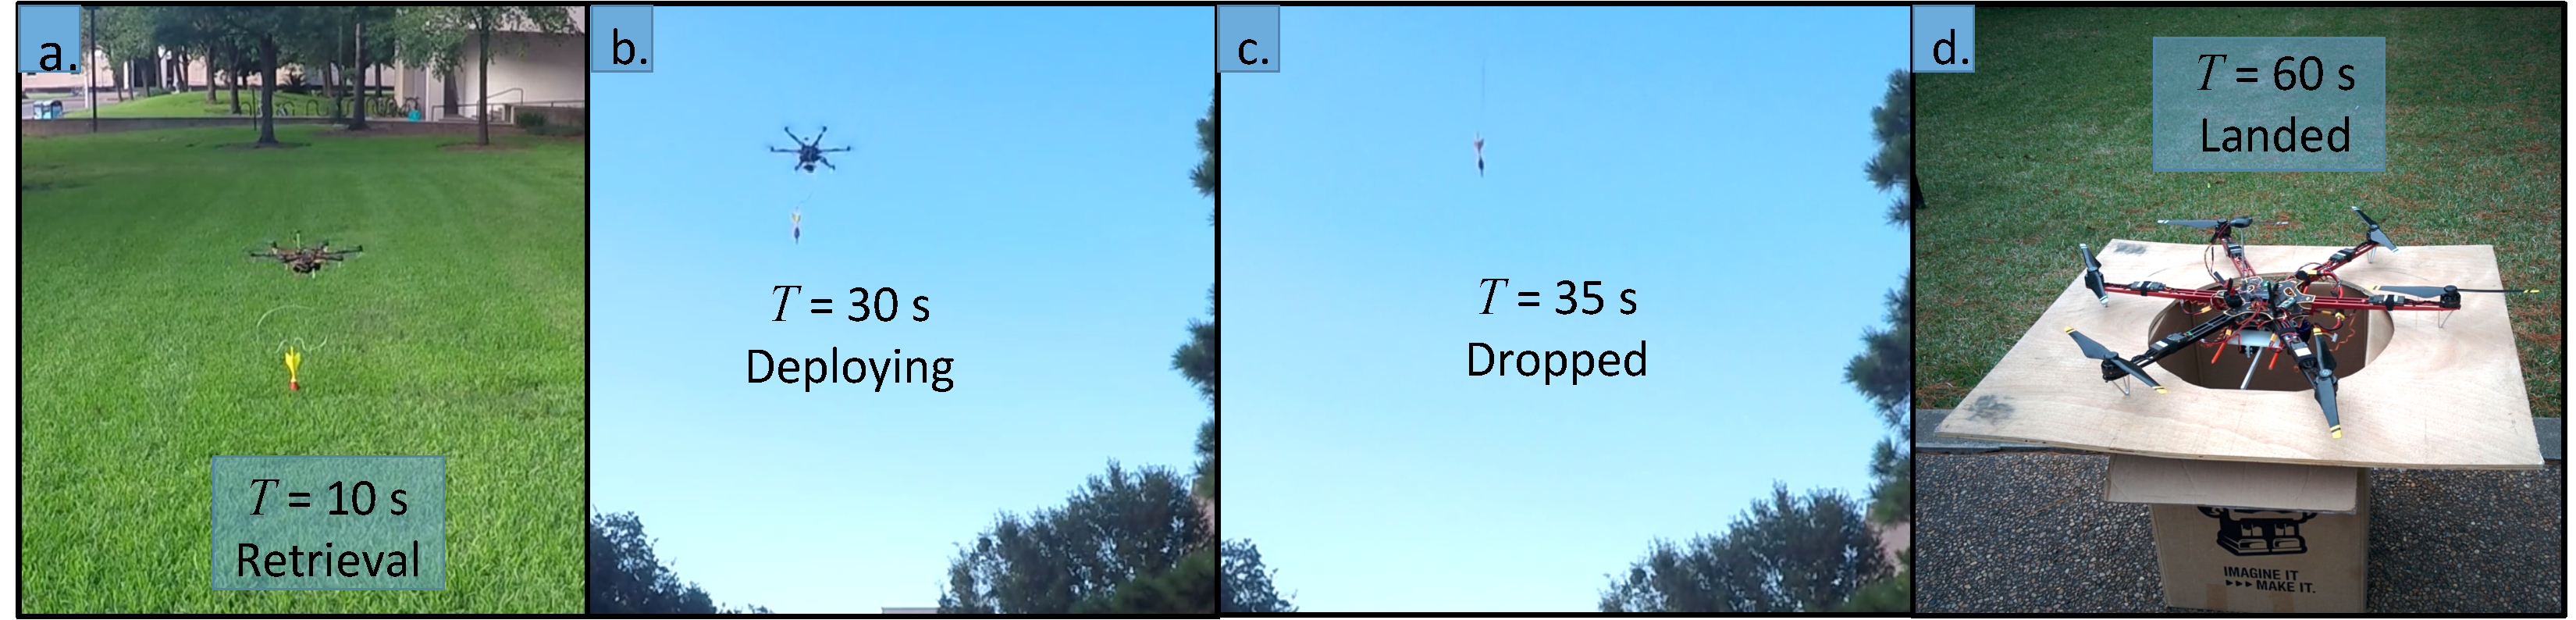
\includegraphics[width=\columnwidth]{SeismicDart_DR.pdf}}
 \caption{SmartDart retrieval and redeployment  See video  attachment. 
 \label{fig:SeismicDart_DR}}
\end{figure}
 
%
\section{SeismicSpider}\label{sec:SeismicSpider}

\subsection{Design}

\subsection{Experiments}
\subsubsection{Exp 1: Accuracy plot}
Hexapod move to desired GPS location  (plot accuracy)\\
\subsubsection{Exp 2: Shot gather comparison}
Hexapod sensing accuracy vs ground setup\\
\subsubsection{Exp 3: Deploying and Retrieving Hexapod}
Exp 5: Retrieving Hexapod\\
%
\section{DeploymentUnit(UAV)}\label{sec:DeploymentUnit(UAV)}

\subsection{Design}
Task Allocation Theory : I want to explore how to assign k smart darts, m hexapods, and n drones  (k=500,m=20, n = 10).  
How should we assign them?  
What changes as k,m,n shift?
Can we write this as a linear program?
Can we reuse Srikanth’s old code, but adapt it for 3D topology?

%
\section{Comparision}\label{sec:Comparision}

\subsection{Ballistic Deployment}
See Fig.~\ref{fig:TradvsAutoDrop}.
\todobox{Need text for this}

\begin{figure} \centering
  {\includegraphics[width=\columnwidth]{PotatoCannon.png}}
 \caption{A pneumatic launcher for SeismicDarts.  Ballistic dart deployment has limited usefulness because the incident angle is equal to the firing angle.} 
 \label{fig:TradvsAutoDrop}
\end{figure}



\subsection{Simulation Studies}

A scheduling system to compare  time and costs for seismic surveys with varying numbers of Deployment Units, SeismicSpiders, SmartDarts, and Human manual laborers was coded in  {\sc Matlab}, available at \cite{Srikanth2016seismicScheduler}.

This tool allows us to examine engineering and logistic tradeoffs quickly in simulation.  For example, Fig.~\ref{fig:DronevsTime} assumes a fixed number of darts (5000), and examines the finishing time with 5 to 500 UAVs.  The time required decays asymptotically, but  XX drones requires only 5\% more time than 5000 drones, indicating that XX are sufficient for the task. Lines are also plotted for XX,XX, and XX total darts.  In each case, substantial cost savings can be obtained by selecting the number of drones required to complete within 5\% of the optimal time.
The tool is useful for comparing the effectiveness of heterogeneous teams.  Table XX compares surveying a 1 km x 10 km strip of land with team (a) XX drones, (b) XX SeismicSpiders and XX drones, (c) XX humans.  Team (a) completed XX times faster than team (c).

\begin{figure*}
\centering
\renewcommand{\figwid}{0.5\columnwidth}
\begin{overpic}[width =\figwid]{sim1_1.pdf}
\end{overpic}
\begin{overpic}[width =\figwid]{sim1_2.pdf}
\end{overpic}
\begin{overpic}[width =\figwid]{sim1_3.pdf}
\end{overpic}
\begin{overpic}[width =\figwid]{sim1_4.pdf}
\end{overpic}

\caption{Simulations were performed to estimate time take by different sensors a.) Only seismic spiders b.) Smart darts and deployment system c.) Heterogeneous System d.) Human workers
\label{fig:Sim_overview}}
\end{figure*}
\begin{figure} \centering
  {\includegraphics[width=\columnwidth]{simulation_table.pdf}}
 \caption{Simulations were performed to estimate time take by different sensors a.) Only seismic spiders b.) Smart darts and deployment system c.) Heterogeneous System d.) Human workers} 
 \label{fig:TradvsAutoDrop}
\end{figure}
\begin{figure} \centering
  {\includegraphics[width=\columnwidth]{DronevsTime.pdf}}
 \caption{This plot captures no. of drones vs time taken.} 
 \label{fig:DronevsTime}
\end{figure}
\begin{figure} \centering
  {\includegraphics[width=\columnwidth]{het_sen_ratio.pdf}}
 \caption{This plot captures time with respect to different sensor ratios. The total number of sensors \{5000,3000\} were kept constant. UAVs were taken to be 10\% of darts for this experiment. } 
 \label{fig:DronevsTime}
\end{figure}
%
 \section{Conclusion and FutureWork}\label{sec:Conclusion}



\bibliographystyle{IEEEtran}
\bibliography{./bibs/Match}

% that's all folks
\end{document}


